% !TEX root = saveliev_physics_general_course_1.tex
%!TEX TS-program = pdflatex
%!TEX encoding = UTF-8 Unicode


\chapter{THE CRYSTALLINE STATE}\label{chap:13}

\section{Features of the Crystalline State}\label{sec:13_1}

The majority of solids in nature have a crystalline structure. For example, almost all minerals and all metals in the solid state are crystals.

A feature of the crystalline state distinguishing it from the fluid states is the presence of \textbf{anisotropy}, \ie, the dependence of a number of physical properties (mechanical, thermal, electrical, optical) on the direction.

Bodies whose properties are identical in all directions are called \textbf{isotropic}. In addition to gases and, with a few exceptions, all liquids, amorphous solids are also isotropic. These solids are supercooled liquids (see Sec.~\ref{sec:15_6}).

The reason why crystals are anisotropic is the ordered arrangement of the particles they are built of (atoms or molecules). The ordered arrangement of the particles manifests itself in the regular external facetting of crystals. Crystals are restricted by plane facets making angles with one another characteristic of a given species of crystals. It is easy to split crystals along definite planes called \textbf{cleavage planes}.

The regularity of the geometrical shape and the anisotropy of crystals do not usually manifest themselves because crystalline bodies are encountered, as a rule, in the form of \textbf{polycrystals}, \ie, conglomerates of a multitude of intergrown, randomly oriented fine crystals. Anisotropy is observed in polycrystals only within the confines of each separately taken minute crystal. A body as a whole does not display anisotropy owing to the chaotic orientation of its crystals. By providing special conditions of crystallization from a melt or a solution, we can obtain large single crystals---\textbf{monocrystals} of any substance. Monocrystals of some minerals are encountered in nature.

The ordered nature of the arrangement of the atoms (or molecules) of a crystal consists in that they are located at the points (or sites) of a geometrically regular space lattice. The entire crystal can be obtained by repeating many times in three different directions the same structural element called an elementary (or unit) crystal cell (\fig{13_1}a). The lengths of the edges $a, b, c$ of a cell are called the \textbf{translation periods} of a crystal.

An elementary cell is a parallelepiped constructed on the three vectors $\vec{a}, \vec{b}, \vec{c}$ whose magnitudes equal the translation periods. This parallelepiped, apart from its edges $a, b, c$, is also characterized by the angles $\alpha, \beta, \gamma$ between the edges (\fig{13_1}b). The quantities $a, b, c$, and $\alpha, \beta, \gamma$ unambiguously define an elementary cell and are called its parameters.

\begin{figure}[t]
	\begin{minipage}[t]{0.5\linewidth}
		\begin{center}
			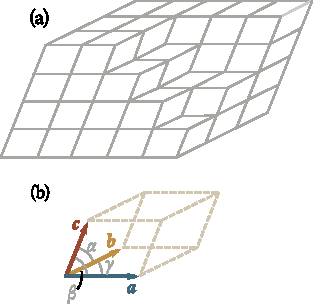
\includegraphics[scale=1]{figures/ch_13/fig_13_1.pdf}
			\caption[]{}
			\label{fig:13_1}
		\end{center}
	\end{minipage}
	\hspace{-0.05cm}
	\begin{minipage}[t]{0.5\linewidth}
		\begin{center}
			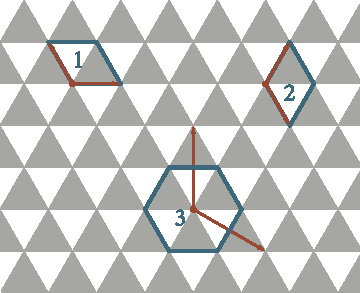
\includegraphics[scale=1]{figures/ch_13/fig_13_2.pdf}
			\caption[]{}
			\label{fig:13_2}
		\end{center}
	\end{minipage}
	\vspace{-0.4cm}
\end{figure}

An elementary cell can be selected in various ways. This is illustrated in \fig{13_2} using an example of a plane structure. The facing of a wall with alternating light and dark triangular tiles can be obtained by repeating different cells many times in two directions (see, for example, cells $1$, $2$, and $3$; the arrows show the directions in which the cells are repeated). Cells $1$ and $2$ are distinguished by including the minimum number of structural elements (one light and one dark tile each). A crystal cell including the smallest number of atoms characterizing the chemical composition of a crystalline substance (for example, one oxygen atom and two hydrogen atoms for an ice crystal) is known as a \textbf{primitive cell}. It is customary practice, however, to select an elementary cell having a greater number of atoms, but with the same symmetry as the entire crystal, instead of a primitive cell. Thus, the plane structure depicted in \fig{13_2} coincides with itself when rotated through \SI{120}{\degree} about any axis at right angles to it that passes through an apex of a tile. Elementary cell $3$ has the same property. Cells $1$ and $2$ have a smaller degree of symmetry: they coincide with themselves only when rotated through \SI{360}{\degree}.

\section{Classification of Crystals}\label{sec:13_2}

A crystal lattice can have different kinds of symmetry. By the symmetry of a crystal lattice is meant its property to coincide with itself upon certain displacements in space.

Every lattice has translation symmetry first of all, \ie, it coincides with itself upon displacement over the translation period\footnote{When considering the symmetry of a lattice, the finite dimensions of the crystal are disregarded, and the lattice is considered to be infinite.}. Among the other kinds of symmetry, we shall note symmetry with respect to rotations about certain axes, and also to mirror reflection relative to definite planes.

If a lattice coincides with itself when rotated about an axis through the angle $2\pi/n$ (consequently, the lattice coincides with itself $n$ times in one complete revolution about the axis), then this axis is called an \textbf{axis of symmetry} of the $n$-th order. It can be shown that apart from the trivial axis of the first order, only axes of symmetry of the second, third, fourth, and sixth orders are possible. Examples of structures having such axes of symmetry are shown schematically in \fig{13_3} (the empty circles, filled circles, and crosses signify atoms of different species).

\begin{figure}[t]
	\begin{center}
		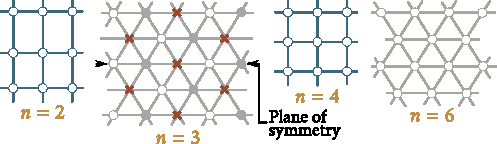
\includegraphics[scale=1.1]{figures/ch_13/fig_13_3.pdf}
		\caption[]{}
		\label{fig:13_3}
	\end{center}
	\vspace{-0.8cm}
\end{figure}

If a lattice coincides with itself when reflected in a certain plane as in a mirror, this plane is defined as a \textbf{plane of symmetry}. An example of a plane of symmetry is also shown in \fig{13_3}.

The different kinds of symmetry are called \textbf{elements of symmetry} of a crystal lattice. There are other elements of symmetry in addition to axes and planes, but we shall not consider them here, however.

A crystal lattice, as a rule, has several kinds of symmetry at a time. Not any combination of the elements of symmetry is possible, however. The prominent Russian scientist Yevgraf Fedorov (1853-1919) showed that $230$ combinations of the symmetry elements are possible. These combinations are called \textbf{space groups}. They are divided according to features of symmetry into $32$ classes. Finally, with respect to the shape of the elementary cell, all crystals are divided into seven \textbf{crystallographic systems}, each of which includes several classes of symmetry.

The crystallographic systems are arranged in the order of growth of their symmetry as follows.
\begin{enumerate}[1.]
	\item \textbf{Triclinic System.} For this system, $a\neq b\neq c$; $\alpha\neq\beta\neq\gamma$. An elementary cell has the form of an oblique parallelepiped.

	\item \textbf{Monoclinic System.} It has two right angles, while the third angle (usually the angle $\beta$) is not a right one. Hence, $a\neq b\neq c$; $\alpha=\gamma=\SI{90}{\degree}, \beta\neq\SI{90}{\degree}$. An elementary cell has the form of a right prism with a parallelogram as its base (\ie, the form of a right parallelepiped).

	\item \textbf{Rhombic System.} All the angles are right ones, all the edges are different: $a\neq b\neq c$; $\alpha=\beta=\gamma=\SI{90}{\degree}$. An elementary cell has the form of a rectangular parallelepiped.

	\item \textbf{Tetragonal System.} All the angles are right ones, two edges are equal: $a=b\neq c$; $\alpha=\beta=\gamma=\SI{90}{\degree}$. An elementary cell has the form of a right prism with a square base.

	\item \textbf{Rhombohedral (or Trigonal) System.} All the edges are equal, all the angles are also equal and are other than right ones: $a=b=c$; $\alpha=\beta=\gamma\neq\SI{90}{\degree}$. An elementary cell has the form of a cube deformed by compression or tension along a diagonal.

	\item \textbf{Hexagonal System.} The edges and the angles between them comply with the conditions $a=b\neq c$; $\alpha=\beta=\SI{90}{\degree}, \gamma=\SI{120}{\degree}$. 	Three elementary cells brought together as shown in \fig{13_4} form a regular hexagonal prism.

	\item \textbf{Cubic System.} All the edges are equal, all the angles are right ones: $a=b=c$; $\alpha=\beta=\gamma=\SI{90}{\degree}$. An elementary cell has the form of a cube.
\end{enumerate}

\section{Physical Kinds of Crystal Lattices}\label{sec:13_3}

Four kinds of crystal lattices and accordingly four kinds of crystals are distinguished depending on the nature of the particles at the lattice points and on the nature of the forces of interaction between the particles. They are ionic, atomic, metallic, and molecular crystals.

\textbf{1. Ionic Crystals.} Ions of opposite signs inhabit the lattice points. The forces of interaction between them are mainly electrostatic (Coulomb). The bond due to the electrostatic forces of attraction between oppositely charged ions is called a \textbf{heteropolar} (or \textbf{ionic}) bond.

A typical example of an ionic lattice is that of table salt (\ce{NaCl}) shown in \fig{13_5}. It belongs to the cubic system. The white circles depict the positively charged sodium ions, and the black circles the negative chloride ions. A glance at the figure shows that the closest neighbours of an ion of a given sign will be ones of the opposite sign. In the gaseous state, \ce{NaCl} consists of molecules in which sodium ions are combined with chloride ones in pairs. The group of an \ce{Na} ion and a \ce{Cl} ion forming a molecule loses its isolated existence in a crystal. An ionic crystal consists of ions, and not of molecules. The entire crystal can be considered as a single giant molecule.

\begin{figure}[t]
	\begin{minipage}[t]{0.5\linewidth}
		\begin{center}
			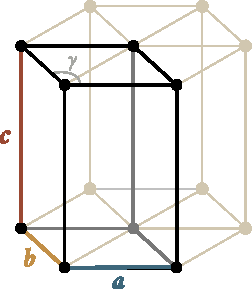
\includegraphics[scale=1.0]{figures/ch_13/fig_13_4.pdf}
			\caption[]{}
			\label{fig:13_4}
		\end{center}
	\end{minipage}
	\hspace{-0.05cm}
	\begin{minipage}[t]{0.5\linewidth}
		\begin{center}
			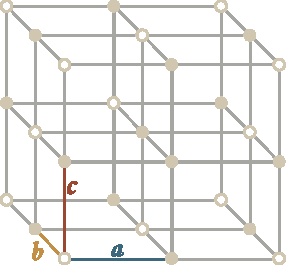
\includegraphics[scale=1.0]{figures/ch_13/fig_13_5.pdf}
			\caption[]{}
			\label{fig:13_5}
		\end{center}
	\end{minipage}
	\vspace{-0.4cm}
\end{figure}

\textbf{2. Atomic Crystals.} The lattice points accommodate neutral atoms. The bond between neutral atoms in a crystal (and also in a molecule) is called \textbf{homopolar} (or \textbf{covalent}). The forces of interaction with a homopolar bond are also of an electrical (but not of a Coulomb) nature. These forces can be explained only on the basis of quantum mechanics.

A homopolar bond is produced by electron pairs. This signifies that one electron from each atom participates in setting up a bond between two atoms. For this reason, a homopolar bond has a directed nature. In a heteropolar bond, each ion acts on all the ions that are sufficiently close to it. In a homopolar bond, the action is directed toward the atom with which the given one shares an electron pair. A homopolar bond can be set up only by valence electrons, whose bond to the atom is the weakest. Since each electron can set up a bond with only one atom, the number of bonds which a given atom can participate in (the number of neighbours with which it can be bound) equals its valence.

Typical examples of atomic crystals are diamond and graphite. The chemical nature of these two substances is the same (they are both constructed of carbon atoms), but they differ in the structure of their crystals. Figure~\ref{fig:13_6}a shows a diamond lattice, and \fig{13_6}b a graphite one. This example clearly shows how the crystal structure of a substance affects its properties.

The typical semiconductors----germanium (\ce{Ge}) and silicon (\ce{Si}) have the same kind of lattice as diamond (a diamond-type lattice). This lattice is characterized by each atom being surrounded by four neighbours at an equal distance from it located at the corners of a regular tetrahedron. Each of the four valence electrons belongs to an electron pair joining this atom with one of its neighbours.

\begin{figure}[t]
	\begin{center}
		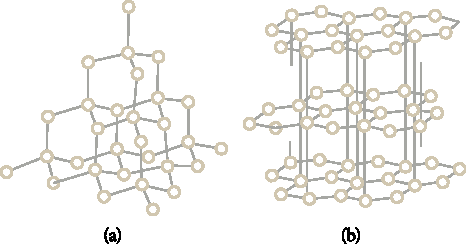
\includegraphics[scale=1.0]{figures/ch_13/fig_13_6.pdf}
		\caption[]{}
		\label{fig:13_6}
	\end{center}
	\vspace{-0.4cm}
\end{figure}

\begin{figure}[t]
	\begin{center}
		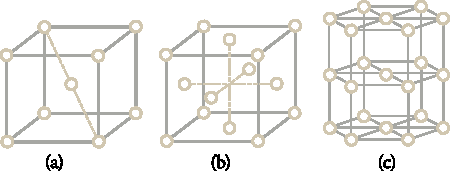
\includegraphics[scale=1.0]{figures/ch_13/fig_13_7.pdf}
		\caption[]{}
		\label{fig:13_7}
	\end{center}
	\vspace{-0.8cm}
\end{figure}

\textbf{3. Metallic Crystals.} Positive ions of the metal are located at all the lattice points. Electrons that detached themselves from the atoms when ions were formed move chaotically between the latter similar to the molecules of a gas. These electrons play the part of a ``cement'' keeping the positive ions together, otherwise the lattice would fall apart under the action of the forces of repulsion between the ions. At the same time, the electrons, in turn, are retained by the ions within the crystal lattice and cannot leave it.

Most metals have lattices of one of three kinds: the cubic volume-centred (\fig{13_7}a), the cubic face-centred (\fig{13_7}b), and the so-called hexagonal close-packed lattice (\fig{13_7}c). The latter is a hexagonal lattice with the ratio $c/a$ equal to $\sqrt{8/3}$. The cubic face-centred and the hexagonal close-packed lattices correspond to the closest packing of identical spheres.

\textbf{4. Molecular Crystals.} Molecules with a definite orientation are located at the lattice points. The forces binding together the molecules in a crystal are of the same nature as the forces of attraction between molecules leading to gases deviating from ideal ones in their properties. This is why they are called \textbf{van der Waals forces}. Molecular lattices are formed, for example, by the following substances: \ce{H2}, \ce{N2}, \ce{02}, \ce{C02}, \ce{H20}. Thus, ordinary ice, and also the so-called dry ice (solid carbon dioxide) are molecular crystals.

\section{Defect in Crystals}\label{sec:13_4}

Defects in crystals are violations of an ideal crystalline structure. Such a violation may consist in the absence of an atom at a lattice point (a vacancy), in the presence of a foreign atom (an impurity atom) instead of an atom of the given substance (a host atom), in the introduction of a surplus atom (host or foreign) into the interstice. Such defects are called \textbf{point} ones. They cause violations in the regularity of a lattice extending over a distance of the order of several periods.

In addition to point defects, there are also defects concentrated near certain lines. They are called \textbf{linear defects} or \textbf{dislocations}. Defects of this kind violate the regular alternation of the crystal planes. The simplest defects of this kind are \textbf{edge} and \textbf{screw} dislocations.

An edge dislocation is due to a surplus crystal half-plane inserted between two adjacent layers of atoms (\fig{13_8}). The edge of this half-plane forms a dislocation of the given kind. The dislocation line is the straight line denoted by the symbol $\perp$ at right angles to the plane of the drawing.

A screw dislocation can be presented as a result of cutting a crystal along a half-plane and the following shifting of the lattice portions at different sides of the cut toward each other over a distance of one period (\fig{13_9}). The internal edge of the cut forms a screw dislocation (see the dash line in the figure). A crystal with a screw dislocation actually consists of a single crystal plane that is curved along a helical surface (such a surface is called a helicoid). The dislocation line coincides with the axis of the screw or helix. The crystal plane is displaced by one period each time it circumvents this line.

\begin{figure}[t]
	\begin{minipage}[t]{0.5\linewidth}
		\begin{center}
			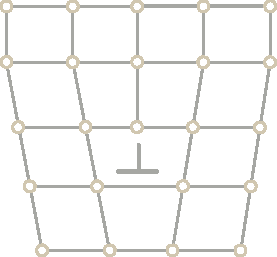
\includegraphics[scale=1.0]{figures/ch_13/fig_13_8.pdf}
			\caption[]{}
			\label{fig:13_8}
		\end{center}
	\end{minipage}
	\hspace{-0.05cm}
	\begin{minipage}[t]{0.5\linewidth}
		\begin{center}
			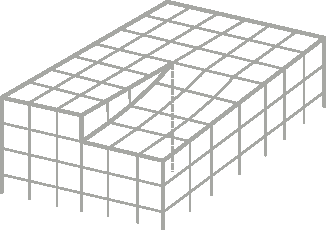
\includegraphics[scale=1.0]{figures/ch_13/fig_13_9.pdf}
			\caption[]{}
			\label{fig:13_9}
		\end{center}
	\end{minipage}
	\vspace{-0.4cm}
\end{figure}

We have considered the two simplest (extreme) kinds of dislocations. In both cases, the dislocation lines are straight. In the general case, these lines may be curved.

Defects greatly affect the physical properties of crystals, including their strength. In particular, dislocations are the reason why the plastic deformation\footnote{A plastic deformation is one that remains after the stress causing it is removed.} of real crystals occurs under the action of stresses that are several orders of magnitude smaller than the stress calculated for ideal crystals.

Shear along the atomic layers readily occurs in the monocrystals of metals. Do not imagine this process in such a way that all the atoms of a layer are displaced simultaneously as a single whole. Actually, the atoms jump over into their new positions in small groups, sequentially. Such a sequential movement of the atoms can be presented as a dislocation movement. The latter requires stresses much smaller than those needed for the displacement of an entire atomic layer at a time. Figure~\ref{fig:13_10} shows the consecutive steps of the process occurring in a crystal under the action of the forces causing the shear. The initially present dislocation under the action of the stresses set up in the crystal moves along the latter. This movement is attended by sequential displacement of the atoms in the layer above the dislocation relative to the atoms of the layer under it.

Dislocation movements are prevented by the presence of other defects in a crystal, for example, by the presence of impurity atoms. Dislocations are also inhibited when they intersect. If the number of dislocations and other defects in a crystal is small, the dislocations spread virtually without hindrance. As a result, the resistance to shear will not be great. An increase in the density of the dislocations and a growth in the concentration of the impurities lead to great inhibition of the dislocations and stopping of their spreading. As a result, the strength of the material grows. For example, the strength of iron is increased by dissolving carbon atoms in it (steel is such a solution).

Plastic deformation is attended by the destruction of the crystal lattice and the formation of a great number of defects preventing the spreading of the dislocations. This explains why metals are hardened upon their cold working.

\begin{figure}[t]
	\begin{center}
		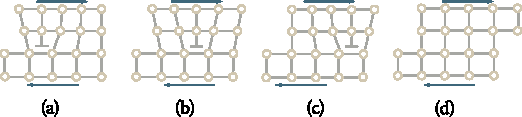
\includegraphics[scale=1.0]{figures/ch_13/fig_13_10.pdf}
		\caption[]{}
		\label{fig:13_10}
	\end{center}
	\vspace{-0.8cm}
\end{figure}

A screw dislocation often appears in the course of the growth of a crystal from a solution or melt. The capture of an atom by a smooth flat crystal surface is less profitable from the energy viewpoint and is therefore less probable than the attachment of an atom to a step on the surface of a crystal with a screw dislocation. This is why it is preferable practice to grow crystals with a screw dislocation built into them. New atoms attach themselves to the edge of the step, owing to which the crystal grows along a spiral.

\section{Heat Capacity of Crystals}\label{sec:13_5}

The location of particles at the points of a crystal lattice corresponds to a minimum of their mutual potential energy. When particles are displaced from their equilibrium position in any direction, a force appears that tends to return them to their initial position. As a result, oscillations of the particles begin. Oscillation in an arbitrary direction can be represented as the superposition of oscillations in three mutually perpendicular directions. Therefore, three vibrational degrees of freedom should be ascribed to every particle in a crystal.

We learned in Sec.~\ref{sec:11_5} that an energy equal to two halves of $kT$---one half in the form of kinetic and the other in the form of potential energy---falls on the average to each vibrational degree of freedom. Consequently, an energy equal to $3kT$ falls on the average to every particle---every atom in an atomic lattice, every ion in an ionic or metallic lattice\footnote{Matters are more complicated for molecular crystals. The molecules in addition to translational oscillations also perform torsional oscillations. Apart from this, the atoms oscillate inside the molecules.}. We can find the energy of a mole of a substance in the crystalline state by multiplying the mean energy of one particle by the number of particles at the points of the crystal lattice. The latter number coincides with the Avogadro constant $\ab{N}{A}$ only for chemically simple substances. For a diatomic substance such as \ce{NaCl}, the number of particles will be $2\ab{N}{A}$ because a mole of \ce{NaCl} contains $\ab{N}{A}$ atoms of \ce{Na} and $\ab{N}{A}$ atoms of \ce{Cl}, for a triatomic one it will be $3\ab{N}{A}$ and so on.

Restricting ourselves to a consideration of chemically simple substances forming atomic or metallic crystals, we can write the following expression for the internal energy of a mole of a substance in the crystalline state:
\begin{equation*}
	\ab{U}{m} = \ab{N}{A} 3kT = 3RT.
\end{equation*}

The increment of the internal energy corresponding to elevation of the temperature by one kelvin, according to \eqn{12_53}, equals the heat capacity at constant volume. Hence,
\begin{equation}\label{eq:13_1}
	C_V = 3R.
\end{equation}

\noindent
Since the volume of solids changes only slightly when they are heated, their heat capacity at constant pressure insignificantly differs from the heat capacity at constant volume; we can therefore assume that $C_p\approx C_V$ and speak simply of the heat capacity of a solid.

Thus, \eqn{13_1} states that the molar heat capacity of chemically simple bodies in the crystalline state is the same and equals $3R$. This statement is the content of the \textbf{Dulong and Petit law} established experimentally. This law is obeyed with quite a good approximation for many substances at room temperature. There are exceptions to this law, however. For example, diamond has a heat capacity of only about $0.7R$ at room temperature.

\begin{figure}[t]
	\begin{center}
		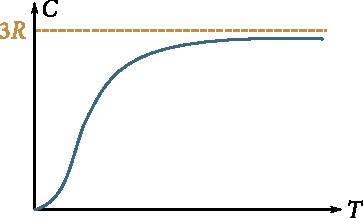
\includegraphics[scale=1.0]{figures/ch_13/fig_13_11.pdf}
		\caption[]{}
		\label{fig:13_11}
	\end{center}
	\vspace{-0.8cm}
\end{figure}

Moreover, notwithstanding \eqn{13_1}, the heat capacity of crystals depends on the temperature, this dependence having the nature shown in \fig{13_11}. Near absolute zero, the heat capacity of all bodies is proportional to $T^3$, and only at a sufficiently high temperature characteristic of each substance does \eqn{13_1} begin to be obeyed. For most substances, this already occurs at room temperature. But for diamond the heat capacity only reaches the value of $3R$ at a temperature of about \SI{1000}{\degreeCelsius}.

The strict theory of the heat capacity of solids proposed by A. Einstein and P. Debye takes into account, first, the quantization of the energy of vibrational motion (see Sec.~\ref{sec:11_5}). Second, the theory takes into account that the oscillations of the particles in a crystal lattice are not independent. This theory, which we shall set out in Volume 3, is in good agreement with experimental data. In particular, for high temperatures, it leads to \eqn{13_1}.
